\begin{landscape}
	\section{Class Diagram}
	
	\begin{figure}[H]
		\centering
		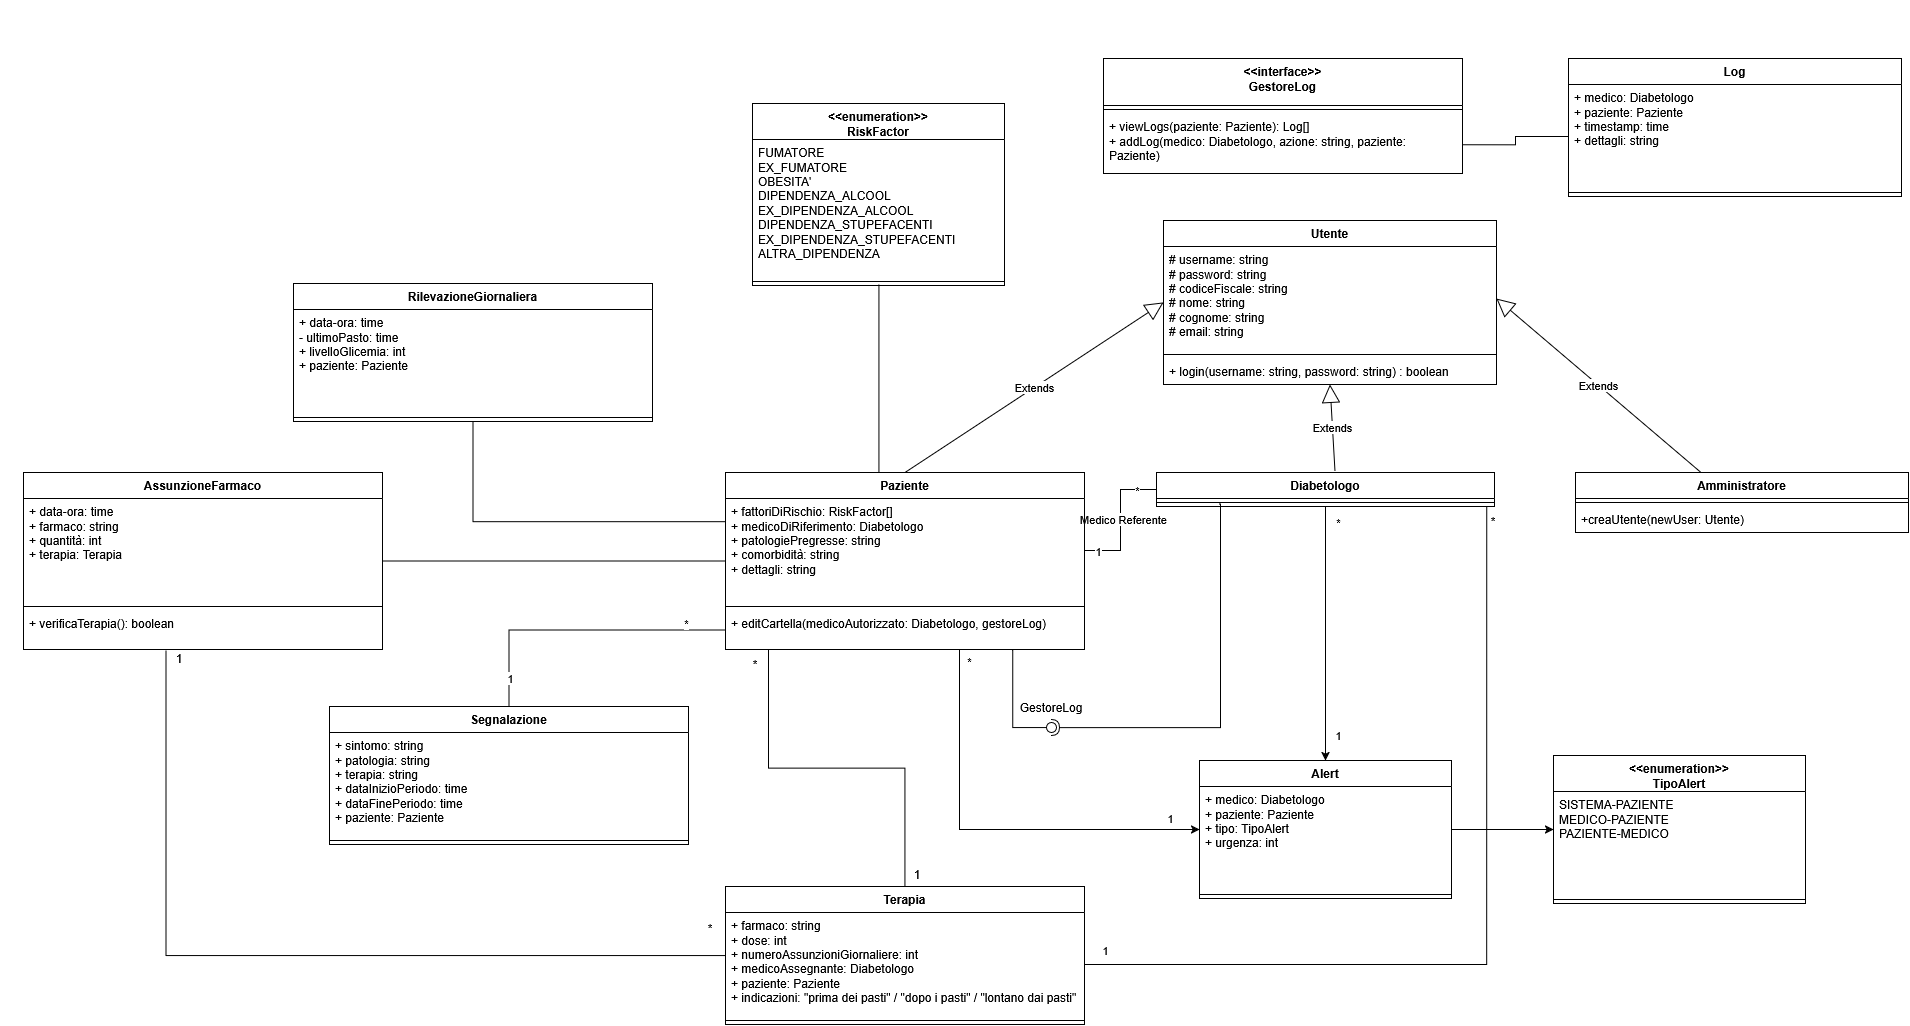
\includegraphics[
		width=1\linewidth,
		height=0.99\textheight,
		keepaspectratio
		]{Immagini/Bozza-UML(6).drawio.png}
		\caption{Class Diagram}
		\label{fig:class-diagram}
	\end{figure}
\end{landscape}

\clearpage

\subsection{Class Diagram della modellazione concettuale}

Il sistema è incentrato sulla classe astratta Utente, raccoglie i dati comuni ai diversi tipi di utilizzatori, quali username, password, codice fiscale, nome, cognome ed email. Da essa derivano le classi Paziente, Diabetologo e Responsabile.\\

A ogni Paziente è associato un Diabetologo come medico di riferimento. Il Paziente mantiene inoltre i propri fattori di rischio, rappresentati tramite  l'enumerazione RiskFactor, oltre che le proprie patologie pregresse, comorbidità e altri dettagli clinici. La modifica della cartella clinica (editCartella()) richiede l'autorizzazione di un medico e viene registrata tramite l'interfaccia GestoreLog, che salva ogni operazione in un oggetto Log (medico, paziente, timestamp, dettagli), in modo da assicurare il requisito di tracciabilità delle operazioni dei medici.\\
Le rilevazioni giornaliere registrano data e ora, ultimo pasto e livello di glicemia. Le assunzioni di farmaci sono verificate rispetto alla Terapia assegnata tramite verificaTerapia().\\
Il paziente può inoltre effettuare Segnalazioni relative a sintomi, patologie o altre situazioni rilevanti. Il sistema gestisce messaggi tra paziente e diabetologo e genera messaggi di sistema destinati al paziente o al medico in presenza di condizioni che richiedono attenzione, come valori glicemici fuori soglia o mancata aderenza alla terapia.\\

Il Diabetologo può visualizzare i pazienti di propria competenza, consultare il loro andamento glicemico e gestire le relative terapie e informazioni cliniche.
La classe Terapia contiene le informazioni relative al farmaco prescritto, alla dose, al numero di assunzioni giornaliere, al medico assegnante e alle indicazioni. Una stessa terapia può essere associata a più pazienti. Quando una terapia condivisa viene modificata per un singolo paziente, viene creata una nuova terapia per evitare di modificare quella degli altri pazienti.\\

Il Responsabile è incaricato della gestione degli utenti del sistema, in particolare della creazione e modifica dei dati relativi a pazienti e diabetologi.\\

La persistenza dei dati è garantita dalla classe Database, che centralizza il caricamento, il salvataggio, l'inserimento, la modifica e il recupero delle informazioni memorizzate nel file del database.

\begin{landscape}
	\section{Class Diagram del software}
	
	\begin{figure}[H]
		\centering
		\includesvg[
		width=0.99\linewidth,
		height=0.99\textheight,
		keepaspectratio
		]{Immagini/UmlSpecifico}
		\caption{Class Diagram del software}
		\label{fig:class-diagram-software}
	\end{figure}
\end{landscape}

\clearpage

 \textcolor{red}{TODO: METTERE}
